\documentclass{article}
\usepackage[utf8]{inputenc}
\usepackage[T1]{fontenc}
\usepackage[brazil]{babel}
\usepackage{geometry}
\usepackage{setspace}
\usepackage[scaled]{helvet} 
\renewcommand\familydefault{\sfdefault} % Define Arial como padrão
\usepackage{pgfplots}
\pgfplotsset{compat=1.18}
\usepackage{tikz}
\usepackage{graphicx}
\usepackage{booktabs}
\usepackage{indentfirst}
\usepackage{float}
\usepackage{amsmath}
\usepackage{amssymb}
\usepackage{amsfonts}
\usepackage{titlesec}
\usepackage{enumitem}
\usepackage{tabularx}
\usepackage{multirow}
\usepackage{url}
\usepackage{ulem}
\usepackage{cite}
\usepackage{balance}
\usepackage{textcomp}
\usepackage{xcolor}
\usepackage{caption}
\usepackage{subcaption}
\usepackage{algorithm}
\usepackage{algpseudocode}

\floatname{algorithm}{Algoritmo}
% --- Pacote para os Pontinhos no Sumário ---
\usepackage{tocloft}
\renewcommand{\cftsecleader}{\cftdotfill{\cftdotsep}}

% --- Configuração de Margens (Padrão PUCPR - Word Template) ---
\geometry{
    top=3.0cm,
    left=3.0cm,
    bottom=2.0cm,
    right=2.0cm
}

% --- Espaçamento e Recuo ---
\onehalfspacing 
\setlength{\parindent}{1.5cm}

% --- Configuração de Títulos ---
\titleformat{\section}{\bfseries\uppercase}{\thesection}{1em}{}
\titleformat{\subsection}{\bfseries}{\thesubsection}{1em}{}

% --- Ajuste de nomes para o Babel ---
\addto\captionsbrazil{\renewcommand{\contentsname}{}}

\makeatletter
\renewcommand{\tableofcontents}{%
    \@starttoc{toc}%
}
\makeatother

\begin{document}

% ============================================================================
% CAPA
% ============================================================================
\thispagestyle{empty}

\noindent 
\begin{minipage}[c]{0.22\textwidth}
    \includegraphics[width=\linewidth]{images/Logo.png} 
\end{minipage}%
\hfill 
\begin{minipage}[c]{0.75\textwidth}
    \centering
    \textbf{
    PONTIFÍCIA UNIVERSIDADE CATÓLICA DO PARANÁ\\
    PRÓ-REITORIA DE PESQUISA, PÓS-GRADUAÇÃO E \hfill INOVAÇÃO\\
    PROGRAMA INSTITUCIONAL DE BOLSAS DE INICIAÇÃO CIENTÍFICA – PIBIC
    }
\end{minipage}

\vspace{4cm}

\begin{center}
    \textbf{RELATÓRIO FINAL}
    
    \vspace{2.5cm}

    \textbf{FUSÃO DE REPRESENTAÇÕES PARA ADAPTAÇÃO DE DOMÍNIO DE MODELOS
PROFUNDOS NO MONITORAMENTO INTELIGENTE DE VAGAS DE
ESTACIONAMENTO} \\
    
    \vspace{\fill}

    \textbf{CURITIBA} \\
    \textbf{2026}
\end{center}
\newpage

% ============================================================================
% FOLHA DE ROSTO
% ============================================================================
\thispagestyle{empty}

\begin{center}
    \textbf{Lucas de Oliveira Cunha} \\
    \textbf{André Gustavo Hochuli} \\
    \textbf{Ciências da Computação- Escola Politécnica}
    
    \vspace{2cm}
    
    \textbf{FUSÃO DE REPRESENTAÇÕES PARA ADAPTAÇÃO DE DOMÍNIO DE MODELOS
PROFUNDOS NO MONITORAMENTO INTELIGENTE DE VAGAS DE
ESTACIONAMENTO}
\end{center}

\vspace{3cm}

\begin{flushright}
    \begin{minipage}{0.5\textwidth}
        \setstretch{1.0} \small
        Relatório Final apresentado ao Programa Institucional de Bolsas de Iniciação Científica e Tecnológica, Pró-Reitoria de Pesquisa, Pós-Graduação e Inovação da Pontifícia Universidade Católica do Paraná. \\
        \textbf{Orientador:} André Gustavo Hochuli
    \end{minipage}
    
\end{flushright}

\vspace{\fill}

\begin{center}
    \textbf{CURITIBA} \\
    \textbf{2026}
\end{center}

\newpage
\begin{center}
    \textbf{Resumo}
    
\end{center}

Este trabalho aprofunda e detalha os resultados obtidos na vigência do PIBIC 2025-2026, que fundamentaram o artigo aceito na SMC: "Ensemble-Based Self-Taught Learning Approach for Parking Space Classification under Limited Data". Propõe-se uma abordagem de aprendizado autodidata (\textit{self-taught learning}) baseada em um \textit{ensemble} de \textit{Convolutional Autoencoders} (CAE) para a classificação de vagas de estacionamento sob restrição de dados anotados. Os experimentos, conduzidos nos \textit{datasets} PKLot e CNR-EXT sob protocolo de avaliação \textit{cross-dataset}, demonstram que a arquitetura CAE supera consistentemente a arquitetura \textit{Variational Autoencoder} (VAE) na extração de representações transferíveis. Utilizando apenas 64 amostras rotuladas do domínio-alvo, o método atinge acurácia média de 93\%, alcançando 96,4\% com 1.024 amostras -- resultado competitivo frente a métodos totalmente supervisionados do estado da arte. Além disso, verificou-se que um \textit{ensemble} de 10 \textit{autoencoders} heterogêneos é suficiente para saturar o ganho de desempenho, e que, entre as estratégias de fusão avaliadas (soma, votação, multiplicação e máximo), a fusão de máximo apresentou o melhor desempenho médio combinado entre os dois \textit{datasets} nesse comparativo; a fusão por votação majoritária foi mantida na geração dos resultados finais reportados neste trabalho.

Palavras-chave: 1. Visão computacional; 2. Dados limitados; 3. Aprendizado de máquina; 4. Ensemble; 5. Aprendizado profundo.

\newpage


% ============================================================================
% SUMÁRIO
% ============================================================================
\newpage
\begin{center}
    \textbf{SUMÁRIO}
\end{center}

\tableofcontents 
\newpage

% ============================================================================
% CONTEÚDO
% ============================================================================
\setcounter{section}{0}

\section{INTRODUÇÃO}\label{sec:introducao}
Com o crescimento urbano impulsionado pelo aumento populacional, a demanda por transporte e automação tem sido cada vez mais necessária. Nesse contexto, a automação de estacionamentos é essencial, dando suporte na gestão, colaborando com o direcionamento exato de vagas disponíveis aos motoristas, otimizando a utilização do espaço e podendo reduzir tempo e dinheiro gastos na busca por vagas\cite{bhattacharya2022review}. 

Na atual literatura, apesar da ampla variedade de tecnologias, as técnicas mais utilizadas são as baseadas em visão computacional e \textit{deep learning}, permitindo que seja empregada em estacionamentos extensos e externos, além de garantir uma ótima performance \cite{Almeida2022, Almeida2023Vehicle}. Entretanto, a grande maioria dessas abordagens são baseadas em cenários específicos com uma grande quantidade de dados anotados e sofrem principalmente com a falta de heterogeneidade nos domínios, limitando-se a imagens muito semelhantes e com pouca diversidade, frequentemente resultando em degradação significativa do desempenho em ambientes não conhecidos \cite{hochuli2023,Luza2025PKLOTDISTILLING}. 

Outro grande desafio sofrido é o alto esforço necessário para coletar e rotular manualmente grandes volumes de imagens \cite{hochuli2022}. A anotação de cenas de estacionamento leva muito tempo e é quase impraticável quando tentamos replicar em outros cenários. Dessa forma, essa limitação motiva paradigmas de aprendizagem que diminuam a dependência de dados rotulados ao mesmo tempo que consigam melhorar a robustez às trocas de domínios. 

Este Relatório Final aprofunda o artigo aceito na SMC, "Ensemble-Based Self-Taught Learning Approach for Parking Space Classification under Limited Data", que apresenta uma versão resumida do método com as decisões de projeto já consolidadas. Em relação ao artigo, este relatório acrescenta, entre outras análises, a justificativa experimental para a escolha da arquitetura CAE em detrimento da VAE (Seção~\ref{subsec:res_unsupervised}) e a comparação entre quatro estratégias de fusão -- soma, votação, multiplicação e máximo (Seção~\ref{subsec:fusao}) --, ao passo que o artigo aceito adota exclusivamente a fusão por votação majoritária, sem explorar ou justificar alternativas.

Nesse sentido, o \textit{Self-Taught Learning} (STL), originalmente proposto por Raina et al.~\cite{Raina2007SelfTaught}, surgiu como uma técnica promissora para diminuir a dependência de dados anotados em larga escala \cite{Delazeri2025Representation,zhang2023STL,vaiyapuri2024STL, germani2023STL}, ao contrário das abordagens totalmente supervisionadas. Nesse método, o STL aprende representações genéricas (como traços, formas e objetos simples) a partir de dados não rotulados e transfere esse aprendizado para o cenário alvo com dados limitados, onde é esperado que mesmo com poucos dados, desempenhe melhor, por já ter um conhecimento prévio. 

Dentro da abordagem STL, a etapa de extração de características exerce um papel fundamental, sendo a principal etapa para o aprendizado genérico. Neste trabalho, iremos explorar diferentes arquiteturas para geração dessas representações, entre elas: \textit{Convolutional Autoencoder (CAE)} e \textit{Variational Autoencoder (VAE)}. Além disso, introduziremos diferentes técnicas de fusão de representações, visando melhorar a robustez da metodologia e a generalização em cenários diversos. 

\section{OBJETIVO}
Este projeto busca analisar soluções que melhorem a adaptação de domínio de
modelos aplicados ao problema de classificação de vagas de estacionamento, implementando técnicas de aprendizado não supervisionado, visando reduzir o esforço
de anotação, otimizar o desempenho do modelo em cenários variados e manter um
baixo custo computacional.

Para alcançar os objetivos propostos, foram definidas as seguintes questões de pesquisa (QPs) que serão abordadas ao longo deste trabalho:

\begin{itemize}
    \item (QP1) Em que medida o aprendizado autodidata (\textbf{\textit{self-taught learning}}) pode reduzir o número de amostras-alvo rotuladas necessárias para alcançar um desempenho competitivo em tarefas de classificação de estacionamentos?
    \item (QP2) Quão robustas são as representações baseadas em STL a mudanças de domínio entre diferentes estacionamentos, em termos de generalização do modelo?
    \item (QP3) Como a abordagem proposta se compara aos métodos de última geração totalmente supervisionados?
        
\end{itemize}
\section{MATERIAIS E MÉTODOS}\label{sec:materiais_metodos}

Nesta seção apresentam-se os materiais e métodos empregados para alcançar os objetivos propostos. Os conceitos e abordagens utilizados são aprofundados nas seções subsequentes.

\subsection{\textit{Convolutional Autoencoder} (CAE)}\label{subsec:autoencoders}

O \textit{Convolutional Autoencoder} (CAE) é um tipo de rede neural não supervisionada treinada para reduzir a dimensionalidade das imagens, aprender representações latentes e reconstruir os dados de entrada. Sua arquitetura divide-se em dois componentes principais:

\begin{itemize}
    \item \textbf{Encoder}: extrai características das imagens, transformando-as em um vetor compactado denominado vetor latente, usando operações de convolução e pooling para produzir essas representações compactadas dos dados de entrada.
    \item \textbf{Decoder}: reconstrói os dados originais a partir do vetor latente, operando de forma inversa ao encoder.
\end{itemize}

\begin{figure}[H]
    \centering
    \includegraphics[width=0.6\linewidth]{images/autoencoder-arc.png}
    \caption{Estrutura do \textit{Convolutional autoencoder}. Fonte: \cite{AutoencoderFigure}}
    \label{fig:autoencoder-arc}
\end{figure}

\subsection{Variational Autoencoder (VAE)}\label{subsec:VAE}

O \textit{Variational Autoencoder} (VAE) \cite{VAE} é um modelo generativo probabilístico que combina \textit{autoencoders} tradicionais com inferência variacional. Diferentemente dos \textit{autoencoders} determinísticos convencionais, nos quais o espaço latente pode tornar-se desorganizado, o VAE aprende uma representação latente contínua e regularizada, permitindo não apenas a reconstrução dos dados, mas também a geração consistente de novas amostras.

O modelo assume que cada dado $x$ é gerado a partir de uma variável latente $z$. Nesse contexto, o encoder não produz uma representação latente determinística direta, mas estima os parâmetros de uma distribuição probabilística sobre o espaço latente. Especificamente, o encoder aprende uma distribuição normal com média $\mu(x)$ e variância $\sigma^2(x)$, assumindo independência entre as dimensões latentes: $z \sim \mathcal{N}(\mu(x), \sigma^2(x))$. A variável latente $z$ é então amostrada dessa distribuição e utilizada pelo decoder para gerar a reconstrução $\hat{x}$.

\begin{figure}[H]
    \centering
    \includegraphics[
            width=0.4\textwidth,
            trim={1cm 2.8cm 1cm 1cm},
            clip
        ]{images/vae-arc.png}
    \caption{Estrutura do \textit{Variational Autoencoder}. Fonte \cite{deeplearningbook2025vae}}
    \label{fig:vae-arc}
\end{figure}

Dessa forma, enquanto o autoencoder clássico aprende uma representação latente determinística, o VAE aprende uma distribuição no espaço latente, modelando explicitamente a incerteza associada à codificação dos dados e impondo uma estrutura probabilística ao espaço latente.

\subsection{Métricas de Avaliação de Reconstrução de Imagens}\label{subsec:metrics}

Para avaliar a qualidade das imagens reconstruídas pelos diferentes autoencoders, empregaram-se métricas quantitativas selecionadas com base em trabalhos da literatura que avaliam GANs e autoencoders em tarefas de reconstrução. Essas métricas auxiliam na identificação da metodologia mais adequada para a geração das representações latentes e, consequentemente, contribuem para responder à \textbf{QP2}. A Tabela \ref{tab:metricas_avaliacao} apresenta as métricas consideradas.

\begin{table}[!h]
\centering
\caption{Métricas de avaliação utilizadas}
\label{tab:metricas_avaliacao}
\begin{tabular}{llll}
\toprule
\textbf{Sigla} & \textbf{Origem} & \textbf{Faixa} & \textbf{Finalidade} \\
\midrule
NCC   & Correlação cruzada normalizada & [-1, 2] & Medir correlação global de intensidade \\
VIF   & Visual Information Fidelity & [0, 2] & Avaliar preservação da informação visual \\
MSE   & Erro quadrático médio & [0, 1] & Quantificar erro pixel a pixel \\
SCC   & Correlação espacial & [-1, 2] & Medir similaridade estrutural espacial \\
PSNR  & Derivada do MSE & $[0, +\infty)$ (dB) & Avaliar qualidade global da reconstrução \\
SSIM  & Métrica perceptual estrutural & [-1, 2] & Avaliar similaridade estrutural entre imagens \\
\bottomrule
\end{tabular}
\end{table}

Ressalta-se que as faixas apresentadas na Tabela \ref{tab:metricas_avaliacao} refletem as formulações estendidas dessas métricas, comumente adotadas na literatura de avaliação de modelos generativos (GANs e \textit{autoencoders}), que permitem valores superiores à unidade em cenários de forte correlação positiva entre a imagem original e a reconstruída. Dessa forma, os valores reportados na Tabela \ref{tab:metrics_reconstruction} (Seção \ref{sec:resultados}) são consistentes com as faixas aqui definidas.

\subsection{Classificadores}\label{subsec:classificadores}

Todos os modelos de classificação foram construídos seguindo uma estrutura padronizada: o \textit{encoder} (como primeira camada), seguido por uma camada de Dropout com taxa de 20\%, duas camadas densas com 256 e 128 unidades e ativação ReLU, e uma camada totalmente conectada de saída com 2 unidades e ativação Softmax.

Essa abordagem permite reutilizar os pesos do encoder previamente treinado de forma não supervisionada (durante 50 épocas), aproveitando sua capacidade de extrair padrões visuais das imagens. Consequentemente, reduz-se o custo computacional do treinamento e o esforço de anotação manual.

O treinamento dos classificadores foi conduzido de forma incremental com o objetivo de responder à \textbf{QP1}, investigando a quantidade mínima de amostras alvo anotadas necessárias para alcançar desempenho competitivo. Para isso, variou-se sistematicamente o número de amostras rotuladas $R$, considerando $R \in \{64, 128, 256, 512, 1024\}$, analisando o impacto dessa variação no desempenho do classificador.

\subsection{Estratégias de Fusão de Representações}\label{subsec:fusao}

Com o objetivo de combinar as informações provenientes dos diferentes classificadores, avaliaram-se quatro estratégias de fusão: soma, votação, multiplicação e máximo. Essas abordagens fundamentam-se na premissa de que a combinação das saídas individuais pode reduzir erros específicos de cada modelo, melhorando consequentemente a robustez e a acurácia geral do sistema. Cada uma das técnicas é descrita a seguir.

\begin{enumerate}
    \item \textbf{Soma}: as probabilidades de saída de cada classificador para uma determinada classe são somadas, e a classe com o maior valor acumulado é selecionada como predição final. Essa técnica assume independência nos erros dos classificadores, buscando suavizar variações individuais e favorecer decisões com consenso entre os modelos, mesmo que parcial.
    
    \item \textbf{Votação}: cada classificador emite um voto correspondente à classe mais provável, sendo a classe final determinada pela maioria dos votos. Trata-se de uma abordagem simples e intuitiva que não depende dos valores de probabilidade, mas apenas da decisão de cada modelo, sendo particularmente útil quando os classificadores apresentam desempenhos similares entre si.
    
    \item \textbf{Multiplicação}: os escores de cada classificador para uma dada classe são multiplicados entre si, e a classe com o maior produto resultante é escolhida. Por sua natureza, essa regra é sensível a valores baixos de probabilidade, de forma que se um classificador atribuir uma probabilidade muito baixa a determinada classe, essa avaliação exerce grande impacto no resultado final, penalizando fortemente discordâncias entre os modelos.
    
    \item \textbf{Máximo}: para cada classe, considera-se o maior escore atribuído entre todos os classificadores, sendo a classe final definida pelo maior valor entre esses máximos. Essa abordagem valoriza a opinião mais confiante entre os modelos, atribuindo a decisão final ao classificador que apresentar a maior certeza (probabilidade) para alguma das classes.
\end{enumerate}

Para aumentar a representatividade da estimativa de desempenho de cada estratégia de fusão, avaliaram-se 50\% de todas as combinações possíveis entre os modelos, partindo de comparações 1 contra 1 até 1 contra todos. Essa amostragem amplia a robustez da média reportada, embora não substitua um teste de significância estatística formal entre as estratégias, conforme discutido na Seção~\ref{sec:discussao}.


\subsection{Conjunto de Dados}\label{subsec:dados}

Para a realização dos experimentos, utilizaram-se os conjuntos de dados PKLot \cite{almeidaEtAl2015} e CNR-EXT \cite{amatoEtAl2017}, que exploram cenários do mundo real com ampla diversificação. Esses datasets permitem a identificação de imagens com variações significativas de brilho, ângulos de captura, obstruções, ambientações e, principalmente, condições climáticas categorizadas em ensolarado, nublado e chuvoso.

\subsubsection{PKLot}

O conjunto de dados PKLot contém 12.417 imagens (1280x720) e 695.899 recortes de vagas de estacionamento, capturados ao longo de 30 dias em intervalos de 5 minutos utilizando uma câmera full-HD de baixo custo (Microsoft LifeCam HD 5000). As imagens foram coletadas em dois estacionamentos: na Universidade Federal do Paraná (UFPR) e na Pontifícia Universidade Católica do Paraná (PUCPR). O dataset está organizado em três subconjuntos: UFPR04, UFPR05 e PUCPR (conforme exemplificado na Figura \ref{fig:overview_pklot}). As câmeras foram posicionadas nos 10º, 4º e 5º andares respectivamente, sendo que no caso da UFPR, as câmeras registraram o mesmo local sob ângulos diferentes.

\begin{figure}[!htbp]
  \centering    
  \subfloat[UFPR04]{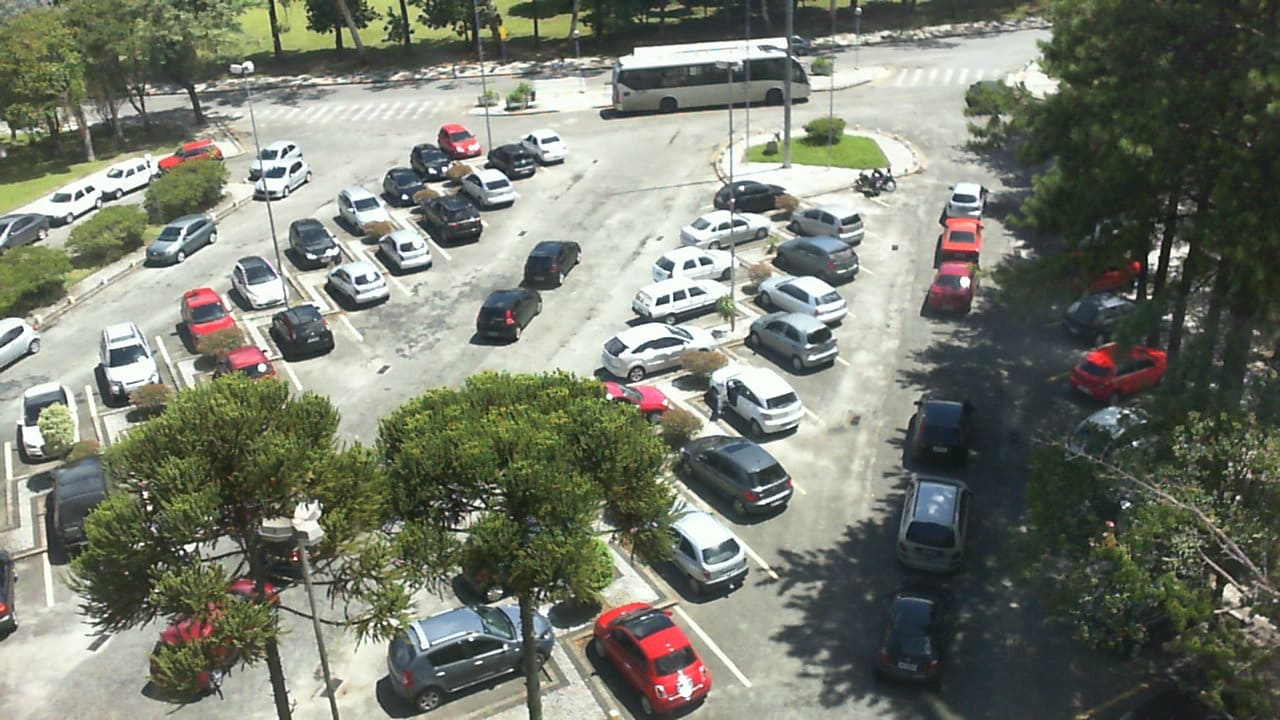
\includegraphics[height=2cm,width=4cm]{images/UFPR04.jpg}}
  \hspace{0.2cm}
  \subfloat[UFPR05]{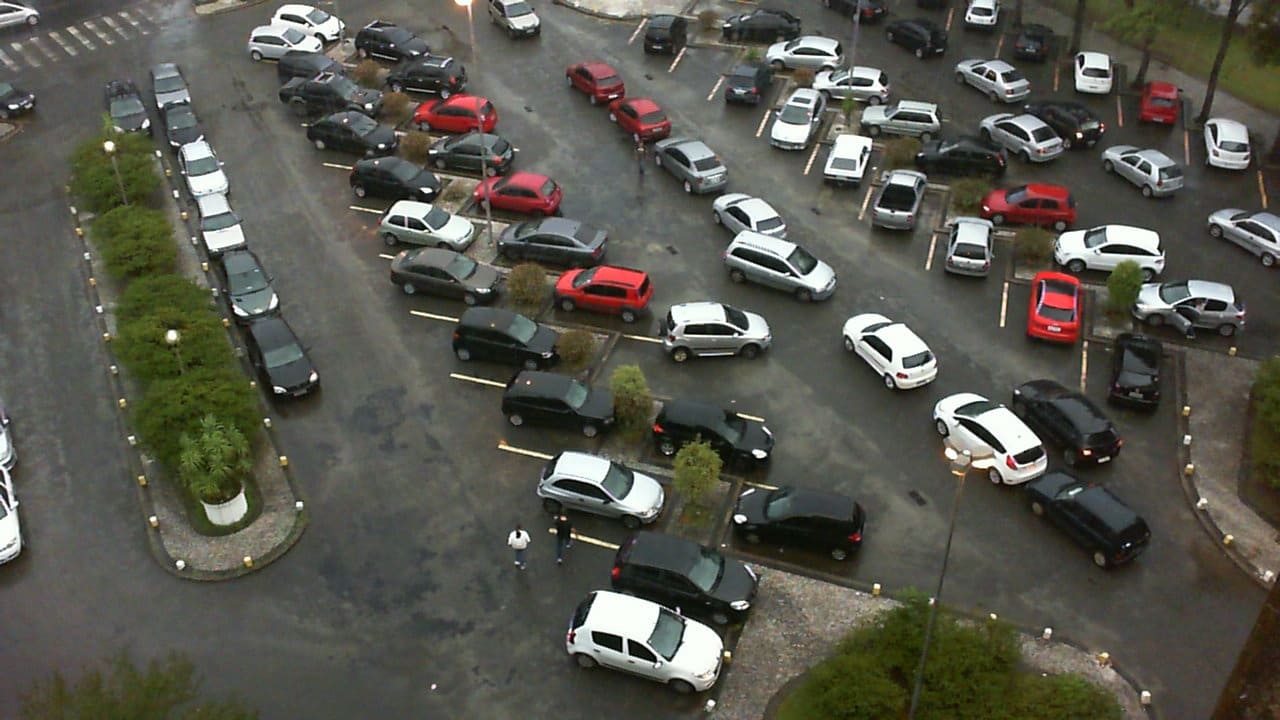
\includegraphics[height=2cm,width=4cm]{images/UFPR05.jpg}}
  \hspace{0.2cm}
  \subfloat[PUCPR]{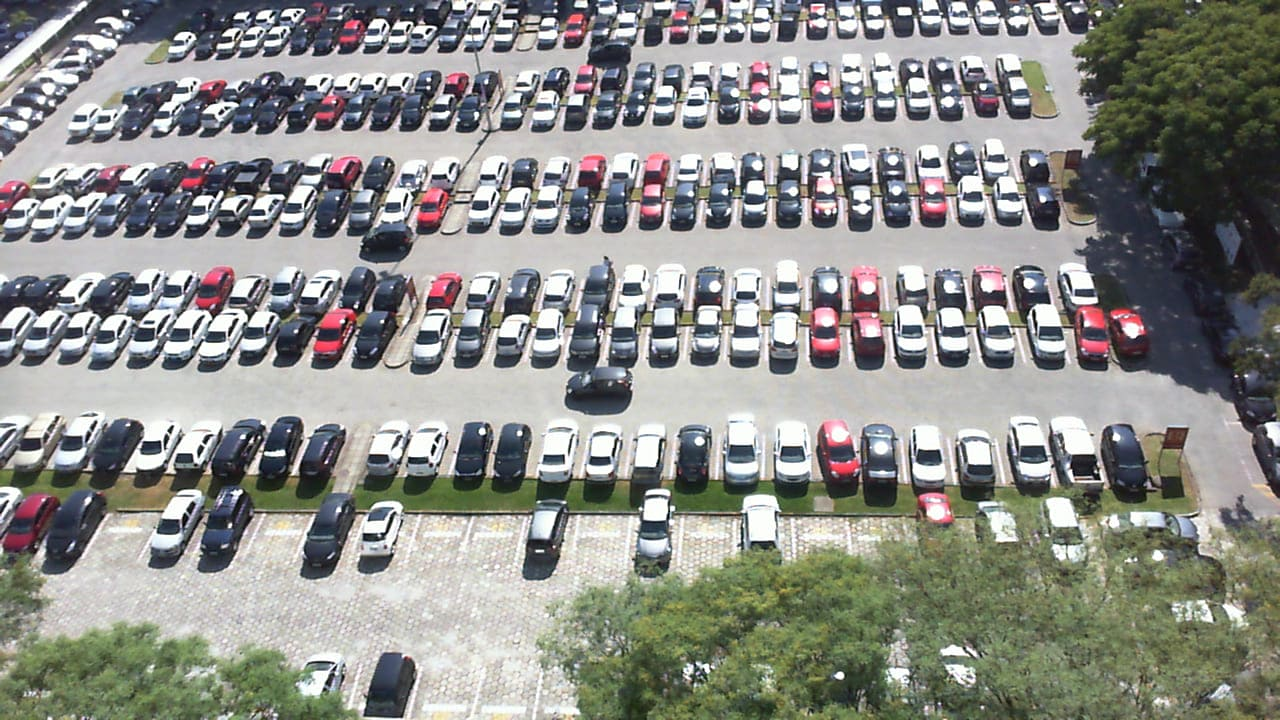
\includegraphics[height=2cm,width=4cm]{images/PUCPR.jpg}}
  \caption{Os três diferentes cenários da PKLot.}
  \label{fig:overview_pklot} 
\end{figure}

\subsubsection{CNR-EXT}

A base de dados CNR-EXT é composta por 4.081 imagens e 157.549 recortes de vagas de estacionamento (256x56), coletadas ao longo de 23 dias entre novembro de 2015 e fevereiro de 2016. Está dividida em nove subconjuntos, cada um identificado por uma câmera em diferentes perspectivas (Figura \ref{fig:overview_cnr}) e ângulos de visão do mesmo estacionamento da National Research Council (CNR), em Pisa, Itália.

\begin{figure}[!ht]
  \centering    
  \subfloat[Camera 1]{\includegraphics[height=2cm,width=4cm]{images/CNR_CAM1.png}}
    \hspace{0.2cm}
  \subfloat[Camera 4]{\includegraphics[height=2cm,width=4cm]{images/CNR_CAM4.png}} 
    \hspace{0.2cm}
  \subfloat[Camera 9]{\includegraphics[height=2cm,width=4cm]{images/CNR_CAM9.png}}
  \caption{Diferentes perspectivas do \textit{dataset} CNR-EXT.}
  \label{fig:overview_cnr}  
\end{figure}



\subsection{Pré-processamento}\label{subsec:preprocessamento}

As imagens foram normalizadas pela divisão dos valores de pixels por 255,0, trazendo-os para o intervalo [0, 1], e redimensionadas para 64x64 pixels. Aplicaram-se técnicas de aumento de dados utilizando a biblioteca Albumentations\cite{albumentations}, modificando as bases apenas durante o treinamento dos classificadores. Especificamente, algumas amostras foram substituídas por versões alteradas com aplicação de efeitos que incluem: chuva, ruído gaussiano, desfoque, permutação de canais de cor, rotação, ajuste de brilho e contraste. A probabilidade de aplicação de qualquer uma dessas transformações foi configurada em 15\% por imagem (Figura \ref{fig:cnr-pklot-dataaug}).

\begin{figure}[H]
    \centering
    \includegraphics[width=0.5\linewidth]{images/cnr-pklot-dataaug.png}
    \caption{Aumento de Dados}
    \label{fig:cnr-pklot-dataaug}
\end{figure}



\subsection{Técnicas de Interpretabilidade}\label{subsec:interpretabilidade}

\subsubsection{Análise por Heatmap}
A análise das regiões mais influentes no processo de classificação foi realizada por meio da técnica Grad-CAM \cite{Selvaraju2017GradCAM}, que utiliza os gradientes da classe predita em relação às ativações da última camada convolucional do encoder para gerar um mapa de calor das regiões mais relevantes para a decisão (Figura \ref{fig:heatmap}). Essa abordagem possibilita uma explicação interpretativa das saídas do modelo, facilitando a compreensão das razões subjacentes aos erros de classificação.
\begin{figure}[!h]
    \centering
    \includegraphics[width=1\linewidth]{images/heatmap-example.png}
    \caption{Heatmap dos resultados de classificação}
    \label{fig:heatmap}
\end{figure}


\subsection{Protocolo Experimental}\label{subsec:protocolo}

Nesta seção são descritas as etapas e as decisões metodológicas adotadas para a condução dos experimentos, incluindo a geração e o treinamento dos modelos, a estratégia de divisão dos dados e as justificativas para as escolhas realizadas.

A Figura \ref{fig:pipeline} apresenta uma visão geral do pipeline proposto, dividido em duas etapas complementares. No \textbf{Passo 1}, denominado \textit{Aprendizado não supervisionado de Representações}, um conjunto de Autoencoders Convolucionais (CAEs) é treinado utilizando apenas dados não rotulados provenientes do domínio de origem, com o objetivo de aprender diferentes representações latentes do problema. Em seguida, no \textbf{Passo 2}, denominado \textit{Aprendizado Supervisionado de Tarefas}, os codificadores aprendidos são utilizados como extratores de características para o treinamento de classificadores independentes com um número limitado de amostras rotuladas do domínio-alvo. Por fim, as predições individuais são combinadas por um mecanismo de fusão, produzindo a classificação final entre vagas ocupadas e livres.

Os detalhes do treinamento dos autoencoders são apresentados na Seção \ref{subsubsec:treino_ae}, enquanto o treinamento dos classificadores é descrito na Seção \ref{subsubsec:treino_classif}.

\begin{figure}[H]
    \centering
    \includegraphics[width=0.8\linewidth]{images/pipeline.png}
    \caption{Arquitetura geral da metodologia proposta. O pipeline é composto por duas etapas: (1) aprendizado não supervisionado de representações por meio de um ensemble de Autoencoders Convolucionais; e (2) aprendizado supervisionado de tarefas utilizando os codificadores treinados como extratores de características, seguido da fusão das predições dos classificadores.}
    \label{fig:pipeline}
\end{figure}

\subsubsection{Treinamento dos Autoencoders}\label{subsubsec:treino_ae}

Conforme ilustrado no Passo 1 da Figura \ref{fig:pipeline}, foram gerados dez Autoencoders Convolucionais distintos para compor o ensemble de representações -- arquitetura selecionada em detrimento do \textit{Variational Autoencoder} com base na comparação apresentada na Seção~\ref{subsec:res_unsupervised}. O número de modelos foi definido buscando um equilíbrio entre a diversidade das representações aprendidas e o custo computacional do treinamento. Os modelos foram construídos a partir de uma mesma estrutura-base, na qual diferentes componentes arquiteturais foram definidos estocasticamente, permitindo o aprendizado de representações complementares.

O número de camadas do encoder foi amostrado entre 2 e 5 camadas convolucionais. Para cada camada, o número de filtros foi selecionado aleatoriamente do conjunto $\{8, 16, 32, 64, 128\}$, utilizando convoluções $3\times3$, seguidas da função de ativação ReLU e de uma camada de Dropout com taxa amostrada do conjunto $\{0.2, 0.3, 0.4\}$. Com probabilidade de 50\%, uma operação de MaxPooling podia ser inserida, respeitando o limite máximo de quatro operações ao longo da arquitetura. A dimensão do espaço latente foi amostrada uniformemente no intervalo [128, 2048], enquanto o decoder foi construído de forma simétrica ao encoder.

Os intervalos de busca e os hiperparâmetros adotados foram definidos com base nas recomendações apresentadas por Delazeri et al. \cite{Delazeri2025Representation}. Dessa forma, todos os dez modelos compartilharam a mesma estrutura-base e os mesmos critérios de treinamento, diferenciando-se exclusivamente pelas variações arquiteturais estocásticas, o que favorece o aprendizado de representações complementares e reduz a correlação entre os modelos que compõem o ensemble.

Por fim, durante o treinamento, as amostras foram selecionadas respeitando a distribuição apresentada na Tabela~\ref{tab:datasets}. Ressalta-se que esse total de imagens não rotuladas, compartilhado entre os subgrupos de cada \textit{dataset}, é distinto do número de amostras rotuladas por domínio-alvo utilizado no treinamento dos classificadores (Seção~\ref{subsubsec:treino_classif}), que também pode atingir até 1.024 amostras, porém individualmente por cenário.

\begin{table}[!htbp]
\centering
\caption{Distribuição dos conjuntos de dados utilizados no treinamento dos \textit{Autoencoders}}
\label{tab:datasets}
\begin{tabular}{lccc}
\hline
\textbf{Dataset} & \textbf{Total de Imagens} & \textbf{Subgrupos} & \textbf{Distribuição} \\
\hline
PKLot & 1024 & 3 & 341 (UFPR04), 341 (UFPR05), 342 (PUC) \\
CNR-EXT & 1000 & 9 & 112 (camera1), 111 (cameras 2--9) \\
\hline
\end{tabular}
\end{table}

A seleção dos dias que compõem cada conjunto foi realizada de forma automática, respeitando a exigência mínima de cinco dias distintos para o conjunto PKLot e de dois dias distintos para o conjunto CNR-EXT, garantindo uma distribuição balanceada de imagens entre os subgrupos apresentados na Tabela~\ref{tab:datasets}. Nos casos em que um dia não apresentava imagens suficientes para manter esse equilíbrio, o dia subsequente era automaticamente selecionado para complementar a divisão.

\subsubsection{Treinamento dos Classificadores}\label{subsubsec:treino_classif}

Conforme ilustrado no Passo 2 da Figura \ref{fig:pipeline}, os \textit{encoders} treinados na etapa de aprendizado de representação foram utilizados como extratores de características para o treinamento de classificadores supervisionados independentes. Cada classificador foi treinado exclusivamente sobre as características produzidas pelo \textit{encoder} correspondente, formando um ensemble de classificadores cujas predições são posteriormente combinadas por uma estratégia de fusão para produzir a classificação final. O processo de \textit{fine-tuning} foi realizado durante 10 épocas, considerando a divisão dos dados apresentada na Tabela \ref{tab:split_classificador}.

A construção dos conjuntos de treinamento, validação e teste seguiu um protocolo de divisão temporal, no qual as imagens dos primeiros dias foram utilizadas para treinamento, um dia intermediário foi destinado à validação e os dias subsequentes compuseram o conjunto de teste. Esse protocolo assegura a independência cronológica entre os conjuntos, reduzindo o risco de vazamento de informação e proporcionando uma avaliação mais fiel ao cenário de implantação.

\begin{table}[!htbp]
\centering
\footnotesize
\caption{Separação temporal e quantidade de amostras utilizadas no treinamento dos classificadores.}
\label{tab:split_classificador}

\begin{tabular}{llcccccc}
\toprule
\multirow{2}{*}{\textbf{Dataset}} &
\multirow{2}{*}{\textbf{Subconjunto}} &
\multicolumn{2}{c}{\textbf{Treino}} &
\multicolumn{2}{c}{\textbf{Validação}} &
\multicolumn{2}{c}{\textbf{Teste}} \\
\cmidrule(lr){3-4}
\cmidrule(lr){5-6}
\cmidrule(lr){7-8}
&
& \textbf{Dias} & \textbf{Amostras}
& \textbf{Dias} & \textbf{Amostras}
& \textbf{Dias} & \textbf{Amostras} \\
\midrule

\multirow{3}{*}{PKLot}
& PUC      & 5 & 1024 & 1 & 64 & 32 & 345.936 \\
& UFPR04   & 5 & 1024 & 1 & 64 & 24 & 86.632 \\
& UFPR05   & 5 & 1024 & 1 & 64 & 27 & 133.960 \\

\midrule

\multirow{9}{*}{CNR-EXT}
& Camera1  & 4  & 1024 & 1 & 64 & 9  & 6.055 \\
& Camera2  & 12 & 1024 & 1 & 64 & 5  & 882 \\
& Camera3  & 6  & 1024 & 1 & 64 & 8  & 3.255 \\
& Camera4  & 4  & 1024 & 1 & 64 & 9  & 6.401 \\
& Camera5  & 3  & 1024 & 1 & 64 & 10 & 9.108 \\
& Camera6  & 2  & 1024 & 1 & 64 & 10 & 8.667 \\
& Camera7  & 2  & 1024 & 1 & 64 & 10 & 9.016 \\
& Camera8  & 2  & 1024 & 1 & 64 & 10 & 10.368 \\
& Camera9  & 4  & 1024 & 1 & 64 & 9  & 4.984 \\

\bottomrule
\end{tabular}
\end{table}

\section{RESULTADOS}\label{sec:resultados}

Nesta seção apresentam-se os resultados obtidos durante a condução dos experimentos, seguindo a organização das etapas descritas na Seção \ref{subsec:protocolo}. Os resultados são analisados em duas fases: (1) aprendizado não supervisionado com avaliação de reconstrução, e (2) aprendizado supervisionado com análise de precisão sob diferentes restrições de dados e condições de domínio.

\subsection{Aprendizado não supervisionado}\label{subsec:res_unsupervised}

\subsubsection{Qualidade de Reconstrução dos Autoencoders}

A etapa inicial de avaliação focou em comparar a qualidade das reconstruções obtidas pelos diferentes autoencoders durante o treinamento não supervisionado. A análise da reconstrução revelou limitações práticas que motivaram ajustes na estratégia experimental.

A Tabela \ref{tab:metrics_reconstruction} e a Figura \ref{fig:reconstruction_comparison} apresentam a comparação quantitativa e qualitativa das reconstruções obtidas na base CNR-EXT para os dois modelos utilizados nas etapas subsequentes: o Convolutional Autoencoder (CAE) e o Variational Autoencoder (VAE). Na figura, as imagens originais são exibidas na parte superior, enquanto as respectivas reconstruções são apresentadas na parte inferior.

\begin{table}[htbp]
\centering
\caption{Comparação das métricas de reconstrução na CNR-EXT}
\label{tab:metrics_reconstruction}
\begin{tabular}{lcccccc}
\toprule
\textbf{Modelo} & \textbf{NCC} & \textbf{VIF} & \textbf{MSE} & \textbf{SCC} & \textbf{PSNR} & \textbf{SSIM} \\
\midrule
CAE & 1.777 & 0.174 & 0.0121 & 0.0030 & 44.396 & 1.468 \\
VAE & 1.568 & 0.071 & 0.0222 & -0.0007 & 39.129 & 1.423 \\
\bottomrule
\end{tabular}
\end{table}

Os resultados evidenciam diferenças expressivas entre os modelos avaliados. O Convolutional Autoencoder (CAE) demonstra desempenho superior em praticamente todas as métricas, alcançando valores razoáveis particularmente no PSNR (44.396 dB), indicando boa fidelidade estrutural nas reconstruções. Em contraste, o Variational Autoencoder (VAE) exibe maior degradação na qualidade das reconstruções, refletida tanto nas métricas quantitativas quanto na análise visual. Especificamente, o VAE apresenta os menores valores de VIF e SSIM, sugerindo perda significativa de informação visual durante o processo de reconstrução.

\begin{figure}[H]
\centering

\begin{minipage}{0.45\linewidth}
    \centering
    \includegraphics[
        width=\linewidth,
        trim=24.7cm 0cm 12.1cm 1cm,
        clip
    ]{images/Autoencoder4_CNR_reconstruction.png}
    \caption*{CAE}
\end{minipage}
\hfill
\begin{minipage}{0.45\linewidth}
    \centering
    \includegraphics[
        width=\linewidth,
        trim=24.7cm 0cm 12.1cm 1cm,
        clip
    ]{images/VariationalAutoencoder4_CNR_reconstruction.png}
    \caption*{VAE}
\end{minipage}

\caption{Comparação das reconstruções na base CNR-EXT. Linha superior: imagens originais. Linha inferior: reconstruções obtidas por cada modelo.}
\label{fig:reconstruction_comparison}

\end{figure}


\subsection{Aprendizado Supervisionado de Tarefas}\label{subsec:res_supervised}

\subsubsection{Análise Comparativa entre Arquiteturas de Autoencoder}

Para fundamentar a seleção do modelo base para as etapas subsequentes de fusão, conduziu-se uma análise comparativa de desempenho entre as duas arquiteturas de autoencoder em cenários de fine-tuning com dados limitados. Este teste foi essencial para responder à \textbf{QP2}, identificando qual modelo oferecia representações mais robustas à transferência entre domínios.

A Tabela~\ref{tab:acc_cross_domain} apresenta os resultados de acurácia obtidos com um único par CAE/VAE (arquitetura de índice 0 do gerador estocástico, Seção~\ref{subsubsec:treino_ae}, mantida idêntica entre as duas variantes para garantir comparação controlada), ao variar o número de amostras rotuladas, pré-treinamento não supervisionado na base CNR-EXT, \textit{fine-tuning} na PUC, e avaliação cross-domínio.

\begin{table}[H]
\centering
\caption{Acurácia (\%) da arquitetura de índice 0 CAE/VAE pré-treinados em CNR-EXT, fine-tuned em PUC, avaliados em múltiplos domínios cross-dataset.}
\label{tab:acc_cross_domain}
\resizebox{\textwidth}{!}{
\begin{tabular}{llcccccccccccc}
\toprule
\textbf{Modelo} & \textbf{Amostras} 
& \textbf{PUC} & \textbf{UFPR04} & \textbf{UFPR05} 
& \textbf{CNR-1} & \textbf{CNR-2} & \textbf{CNR-3} & \textbf{CNR-4} & \textbf{CNR-5} 
& \textbf{CNR-6} & \textbf{CNR-7} & \textbf{CNR-8} & \textbf{CNR-9} \\
\midrule
\multirow{5}{*}{\textbf{CAE}}
& 64   & 90,9 & 75,4 & 58,9 & 73,8 & 71,2 & 69,7 & 83,2 & 75,0 & 79,5 & 78,4 & 78,2 & 81,0 \\
& 128  & 94,0 & 78,8 & 59,2 & 75,1 & 77,3 & 70,5 & 82,1 & 81,2 & 81,2 & 80,2 & 81,7 & 82,8 \\
& 256  & 96,6 & 74,1 & 62,8 & 77,6 & 79,6 & 75,9 & 84,5 & 83,3 & 87,3 & 83,3 & 85,2 & 82,0 \\
& 512  & 98,0 & 81,0 & 74,2 & 74,2 & 78,5 & 76,4 & 87,0 & 85,0 & 88,1 & 84,9 & 85,5 & 85,1 \\
& 1024 & 97,4 & 78,1 & 75,6 & 72,7 & 76,6 & 76,4 & 87,8 & 84,7 & 88,6 & 86,7 & 86,1 & 84,1 \\
\midrule
\multirow{5}{*}{\textbf{VAE}}
& 64   & 79,1 & 59,3 & 50,0 & 50,6 & 66,2 & 55,0 & 50,9 & 50,6 & 52,2 & 53,5 & 52,2 & 52,0 \\
& 128  & 80,6 & 67,9 & 53,1 & 50,9 & 63,5 & 52,8 & 51,3 & 50,8 & 51,7 & 54,6 & 52,2 & 51,3 \\
& 256  & 80,9 & 66,3 & 53,1 & 52,7 & 52,6 & 51,5 & 52,7 & 52,0 & 50,3 & 52,5 & 50,9 & 51,2 \\
& 512  & 80,8 & 58,9 & 53,6 & 52,8 & 52,5 & 51,6 & 52,3 & 51,4 & 50,2 & 53,5 & 51,5 & 50,7 \\
& 1024 & 81,0 & 62,3 & 53,5 & 54,5 & 52,3 & 51,5 & 52,7 & 51,7 & 50,1 & 52,7 & 50,9 & 51,7 \\
\bottomrule
\end{tabular}
}
\end{table}

Os resultados evidenciam diferenças substanciais entre as duas arquiteturas. O modelo CAE alcança desempenho robusto mesmo com supervisão limitada, atingindo aproximadamente 91\% de acurácia no domínio PUC com apenas 64 amostras. Conforme aumenta-se o número de amostras rotuladas, o desempenho melhora consistentemente até saturar em torno de 256-512 amostras, com ganhos marginais (<3\%) além deste ponto, indicando que as representações aprendidas pelos encoders já capturam informações suficientemente discriminativas.

Em contraste, o modelo VAE demonstra desempenho significativamente inferior em todos os cenários, com acurácias limitadas entre 50\% e 81\%. Este padrão persistente sugere que a regularização probabilística adicional imposta pelo VAE (que modela o espaço latente como distribuição) dificulta a aprendizagem de representações discriminativas quando dados de treinamento são escassos. Consequentemente, o VAE compromete tanto a acurácia quanto a robustez em cenários de transferência entre domínios.

Com base nesta análise comparativa, o modelo CAE foi selecionado como arquitetura base para as etapas subsequentes de fusão, garantindo que a abordagem proposta partisse de representações efetivas e transferíveis.

\subsubsection{Fusões}

 A Tabela~\ref{tab:fusion_indomain_comparison} apresenta a acurácia das quatro estratégias de fusão avaliadas (máximo, multiplicação, soma e votação) no protocolo in-domain com 10 modelos, variando o número de amostras rotuladas. Os resultados mostram que o \textit{max} lidera em todas as faixas de amostra do CNR-EXT. No PKLot, entretanto, o \textit{max} é superado por multiplicação e soma na maioria das faixas (por exemplo, 89,67\% da multiplicação vs. 89,43\% do max, em média), com margens tipicamente inferiores a 1 ponto percentual. Ainda assim, optou-se por manter a fusão por votação majoritária na geração das demais tabelas de resultados deste trabalho. As diferenças observadas entre as quatro estratégias são pequenas o suficiente para não permitir conclusões fortes sem um teste de significância estatística, o que constitui uma limitação deste trabalho (Seção \ref{sec:discussao}).

\begin{table}[!htbp]
\centering
\footnotesize
\caption{Acurácia (\%) das estratégias de fusão no protocolo \textit{in-domain} (ensemble com 10 modelos).}
\label{tab:fusion_indomain_comparison}

\renewcommand{\arraystretch}{1.05}
\setlength{\tabcolsep}{5pt}

\begin{tabular}{ccccccccc}
\toprule
\multirow{2}{*}{\textbf{Amostras}} &
\multicolumn{4}{c}{\textbf{CNR-EXT}} &
\multicolumn{4}{c}{\textbf{PKLot}} \\
\cmidrule(lr){2-5}
\cmidrule(lr){6-9}
& Max & Mult. & Soma & Voto &
Max & Mult. & Soma & Voto \\
\midrule

64
& \textbf{90,70} & 90,48 & 90,24 & 90,14
& \textbf{85,10} & 83,75 & 83,28 & 82,93 \\

128
& \textbf{91,76} & 91,62 & 91,45 & 91,42
& 87,30 & 88,04 & \textbf{88,15} & 88,08 \\

256
& \textbf{92,49} & 92,46 & 92,37 & 92,33
& 89,78 & 91,14 & \textbf{91,43} & 91,41 \\

512
& \textbf{92,79} & 92,57 & 92,43 & 92,39
& 91,97 & \textbf{92,30} & \textbf{92,30} & 92,27 \\

1024
& \textbf{93,26} & 93,12 & 93,00 & 92,98
& 92,98 & \textbf{93,12} & 93,08 & 93,06 \\

\midrule

\textbf{Média}
& \textbf{92,20} & 92,05 & 91,90 & 91,85
& 89,43 & \textbf{89,67} & 89,65 & 89,55 \\

\bottomrule
\end{tabular}

\end{table}

Quanto ao tamanho do ensemble, a Figura~\ref{fig:ensemble-ablation} mostra que conforme adiciona-se mais modelos, a acurácia melhora, mas esse ganho diminui gradualmente. Por volta de 10 modelos, o desempenho atinge um platô, ou seja, adicionar mais modelos não traz melhoria significativa. Isso significa que 10 autoencoders é o número ideal: suficiente para bom desempenho, mas sem desperdício de recursos computacionais.

\begin{figure}[!htbp]
\centering
\begin{tikzpicture}
\begin{axis}[
    width=\columnwidth,
    height=6.5cm,
    xmin=0.5, xmax=10.8,
    ymin=90, ymax=94,
    xtick={1,3,5,7,9,10},
    ytick={90,91,92,93,94},
    xlabel style={font=\small},
    ylabel style={font=\small},
    xlabel=Tamanho do Ensemble,
    ylabel=Acurácia (\%),
    grid=major,
    grid style={line width=0.2pt, draw=gray!25},
    tick label style={font=\small},
    axis line style={line width=0.8pt},
    legend style={
        at={(0.98,0.30)},
        anchor=east,
        fill=white,
        fill opacity=0.95,
        draw=gray!40,
        font=\footnotesize,
        rounded corners=2pt,
        inner sep=3pt
    },
    every axis plot/.append style={line width=2pt},
]

% CNR baseline (single model)
\addplot[
    dashed,
    color=red!50,
    line width=1.5pt,
] coordinates {(0.5,91.8) (10.8,91.8)};

% PKLot baseline (single model)
\addplot[
    dashed,
    color=blue!50,
    line width=1.5pt,
] coordinates {(0.5,90.6) (10.8,90.6)};

% CNR ensemble
\addplot[
    solid,
    color=red!75!black,
    mark=*,
    mark size=3pt,
] coordinates {
    (3,92.8)
    (5,93.0)
    (7,93.1)
    (9,93.2)
    (10,93.3)
};

% PKLot ensemble
\addplot[
    solid,
    color=blue!75!black,
    mark=*,
    mark size=3pt,
] coordinates {
    (3,92.3)
    (5,92.6)
    (7,92.8)
    (9,92.9)
    (10,93.0)
};

% Single model markers (baseline)
\addplot[
    only marks,
    mark=diamond*,
    mark size=4pt,
    color=red!50,
] coordinates {(1,91.8)};

\addplot[
    only marks,
    mark=diamond*,
    mark size=4pt,
    color=blue!50,
] coordinates {(1,90.6)};

% Labels - CNR baseline
\node[font=\small, color=red!70!black, above right] at (axis cs:1,91.8) {91,8};

% Labels - PKLot baseline
\node[font=\small, color=blue!70!black, below right] at (axis cs:1,90.6) {90,6};

% Labels - CNR ensemble
\node[font=\small, color=red!70!black, above] at (axis cs:3,92.8) {92,8};
\node[font=\small, color=red!70!black, above] at (axis cs:5,93.0) {93,0};
\node[font=\small, color=red!70!black, above] at (axis cs:7,93.1) {93,1};
\node[font=\small, color=red!70!black, above] at (axis cs:9,93.2) {93,2};
\node[font=\small, color=red!70!black, above] at (axis cs:10,93.3) {93,3};

% Labels - PKLot ensemble
\node[font=\small, color=blue!70!black, below] at (axis cs:3,92.3) {92,3};
\node[font=\small, color=blue!70!black, below] at (axis cs:5,92.6) {92,6};
\node[font=\small, color=blue!70!black, below] at (axis cs:7,92.8) {92,8};
\node[font=\small, color=blue!70!black, below] at (axis cs:9,92.9) {92,9};
\node[font=\small, color=blue!70!black, below] at (axis cs:10,93.0) {93,0};

\addlegendentry{CNR-EXT (Ensemble)}
\addlegendentry{PKLot (Ensemble)}
\addlegendentry{Baseline}

\end{axis}
\end{tikzpicture}
\caption{Tamanho do ensemble versus acurácia.}
\label{fig:ensemble-ablation}
\vspace{-3mm}
\end{figure}




\subsubsection{Resultados no Mesmo Domínio}

A Tabela~\ref{tab:batch_vs_base} apresenta os resultados de acurácia obtidos ao aplicar a estratégia proposta, seguindo o protocolo: pré-treinamento não supervisionado em um dataset de representação (CNR-EXT ou PKLot), seguido de \textit{fine-tuning} dos classificadores com amostras rotuladas em número variável (64 a 1024) em um domínio-alvo específico, e avaliação no mesmo domínio utilizado no \textit{fine-tuning}. A predição final é obtida pela fusão por votação majoritária entre os 10 pares \textit{encoder}-classificador do \textit{ensemble}, conforme definido na Seção \ref{subsec:fusao}.

Os resultados validam a efetividade da abordagem. A acurácia melhora consistentemente conforme aumenta-se o número de amostras rotuladas, com diversos cenários atingindo bom desempenho já com 64--128 amostras. Mais importante, o ganho de desempenho se estabiliza a partir de 256 amostras, indicando que adicionar mais dados rotulados resulta em melhorias marginais. Esse padrão de saturação confirma observações anteriores~\cite{SantosPKLOTGAN} e valida a premissa central do aprendizado autodidata: o pré-treinamento não supervisionado fornece uma base sólida, permitindo que o fine-tuning supervisionado converja rapidamente com poucos exemplos.

\begin{table}[!h]
\centering
\caption{Acurácia (\%) dos classificadores em diferentes domínios-alvo conforme o número de amostras rotuladas.}
\label{tab:batch_vs_base}

\footnotesize
\renewcommand{\arraystretch}{0.95}

\begin{tabular}{llccccc}
\toprule
\multirow{2}{*}{\textbf{Representação}} &
\multirow{2}{*}{\textbf{Alvo}} &
\multicolumn{5}{c}{\textbf{Dados rotulados}} \\
\cmidrule(lr){3-7}
 & & 64 & 128 & 256 & 512 & 1024 \\
\midrule

\multirow{3}{*}{CNR}
& PUC    & 95,1 & 97,4 & 98,2 & 98,4 & 98,7 \\
& UFPR04 & 94,0 & 96,3 & 96,5 & 97,0 & 97,4 \\
& UFPR05 & 97,0 & 97,6 & 98,1 & 98,4 & 98,3 \\

\midrule

\multirow{9}{*}{PKLot}
& CNR-1 & 90,7 & 92,6 & 93,7 & 94,3 & 95,8 \\
& CNR-2 & 97,3 & 97,1 & 97,4 & 97,6 & 98,4 \\
& CNR-3 & 95,8 & 94,7 & 96,3 & 97,0 & 97,7 \\
& CNR-4 & 94,7 & 94,5 & 95,1 & 95,0 & 95,4 \\
& CNR-5 & 86,2 & 89,7 & 92,3 & 93,5 & 94,7 \\
& CNR-6 & 92,2 & 92,5 & 93,7 & 93,4 & 95,1 \\
& CNR-7 & 92,3 & 91,8 & 91,1 & 92,0 & 92,9 \\
& CNR-8 & 92,9 & 95,0 & 95,3 & 96,0 & 96,6 \\
& CNR-9 & 91,2 & 91,0 & 92,5 & 94,3 & 95,8 \\

\midrule
\multicolumn{2}{l}{\textbf{Média}} &
\textbf{93,3} &
\textbf{94,2} &
\textbf{95,0} &
\textbf{95,6} &
\textbf{96,4} \\
\bottomrule
\end{tabular}

\end{table}

Cenários com perspectivas mais desafiadoras (câmeras 1 e 9 da Figura \ref{fig:overview_cnr}) demonstram maior sensibilidade ao número de amostras rotuladas, requerendo mais exemplos para atingir desempenho ótimo. No entanto, o desempenho geral permanece estável e competitivo em todos os cenários, demonstrando que a abordagem é robusta e capaz de transferir bem entre diferentes condições de captura.

\subsection{Resultados contra diferentes domínios}

Um aspecto importante para validar a abordagem é avaliar como o modelo generaliza em ambientes novos (QP2). O \textit{ensemble} de 10 \textit{autoencoders}, ajustado com 1.024 amostras rotuladas -- quantidade que resultou no melhor desempenho na avaliação da QP1 -- em um domínio específico, é testado em todos os demais cenários disponíveis, sem qualquer ajuste adicional nos pesos. A decisão final é obtida pela estratégia de fusão por votação majoritária entre os classificadores do \textit{ensemble}, conforme a Seção \ref{subsec:fusao}. Os resultados desta avaliação cross-domínio estão na Tabela~\ref{tab:cross_domain_voting_percent}.

\begin{table*}[!htb]
\centering
\setlength{\tabcolsep}{3pt}
\caption{Desempenho cross-domínio (acurácia em \%). A primeira coluna mostra de qual domínio o classificador foi treinado e as demais colunas mostram como ele se comporta quando testado em outros domínios.}
\label{tab:cross_domain_voting_percent}
\resizebox{0.75\linewidth}{!}{
\begin{tabular}{ccccccccccccc}
\toprule
\multirow{2}{*}{\textbf{\begin{tabular}[c]{@{}c@{}}Classificador \\ Treinado em\end{tabular}}} & \multicolumn{12}{c}{\textbf{Testado em (sem ajustar pesos)}} \\
\cmidrule(lr){2-13}
 & CNR-1 & CNR-2 & CNR-3 & CNR-4 & CNR-5 & CNR-6 & CNR-7 & CNR-8 & CNR-9 & PUC & UFPR04 & UFPR05 \\
\midrule
CNR-1  & 95,8 & 98,1 & 96,5 & 96,1 & 92,0 & 95,7 & 90,9 & 95,7 & 93,7 & 89,2 & 76,9 & 76,6 \\
CNR-2  & 90,5 & 98,4 & 95,2 & 96,3 & 91,4 & 95,8 & 90,3 & 96,2 & 93,8 & 91,2 & 85,4 & 84,1 \\
CNR-3  & 85,9 & 98,0 & 97,7 & 96,0 & 89,0 & 95,1 & 87,3 & 95,9 & 91,5 & 92,3 & 83,0 & 87,4 \\
CNR-4  & 86,3 & 97,2 & 94,1 & 95,4 & 90,8 & 95,3 & 87,7 & 96,5 & 92,7 & 93,7 & 88,3 & 87,4 \\
CNR-5  & 88,5 & 98,3 & 96,3 & 97,2 & 94,7 & 96,1 & 90,7 & 96,8 & 93,8 & 96,6 & 88,4 & 85,4 \\
CNR-6  & 83,1 & 96,5 & 93,0 & 94,5 & 90,1 & 95,1 & 86,0 & 95,5 & 90,1 & 93,8 & 85,5 & 84,2 \\
CNR-7  & 91,1 & 98,1 & 97,7 & 97,6 & 95,4 & 97,2 & 92,9 & 97,3 & 95,4 & 93,3 & 90,1 & 79,4 \\
CNR-8  & 83,0 & 93,9 & 94,6 & 93,7 & 89,5 & 95,3 & 87,3 & 96,6 & 92,0 & 94,8 & 84,7 & 85,7 \\
CNR-9  & 91,1 & 98,0 & 95,4 & 97,3 & 94,0 & 97,0 & 91,0 & 97,6 & 95,8 & 91,8 & 90,1 & 88,2 \\
PUC      & 91,4 & 95,0 & 92,0 & 95,4 & 92,4 & 94,4 & 90,2 & 93,4 & 91,4 & 98,7 & 91,5 & 81,3 \\
UFPR04   & 89,0 & 94,2 & 92,8 & 92,6 & 88,5 & 93,6 & 90,6 & 91,8 & 88,5 & 93,2 & 97,4 & 84,5 \\
UFPR05   & 71,7 & 83,0 & 85,1 & 84,9 & 74,9 & 87,6 & 76,9 & 85,8 & 77,4 & 82,6 & 87,4 & 98,3 \\
\bottomrule
\end{tabular}}
\vspace{-2mm}
\end{table*}

Os resultados mostram que a abordagem funciona bem em cenários cross-domínio. Quando testados em câmeras do mesmo dataset, os classificadores alcançam acurácias altas, indicando que as representações aprendidas são bem transferidas. Por outro lado, quando um modelo treinado em um dataset é testado em outro (por exemplo, CNR-EXT testado em PKLot), a acurácia cai mais, refletindo as diferenças nas condições de captura entre os dois datasets. Mesmo assim, os resultados permanecem competitivos na maioria dos casos, o que valida que o método é robusto o suficiente para funcionar em diferentes cenários reais.

Uma análise mais detalhada da Tabela~\ref{tab:cross_domain_voting_percent} revela que alguns subconjuntos se destacam consistentemente no protocolo cross-domínio, seja como fonte de treinamento, seja como domínio-alvo de teste. Entre os classificadores treinados, CNR-7 e CNR-9 apresentam a maior acurácia média quando avaliados nos demais cenários (93,9\% e 93,8\%, respectivamente), sugerindo que os \textit{encoders} aprendidos a partir dessas câmeras produzem representações mais transferíveis. No caso da câmera 9, uma hipótese explicativa é a maior variedade visual presente em seus dados de treinamento -- particularmente em termos de angulação --, o que possivelmente contribuiu para o aprendizado de representações mais robustas a mudanças de domínio.

Por outro lado, quando considerado como domínio-alvo -- isto é, a facilidade com que classificadores treinados em outros cenários conseguem generalizar para ele --, o subconjunto CNR-4 figura entre os mais bem classificados (94,7\% de acurácia média, atrás apenas de CNR-2, CNR-6 e CNR-8). Uma possível explicação é que a câmera 4 compartilha uma angulação relativamente semelhante à do PKLot e das demais câmeras do CNR-EXT, ao mesmo tempo em que contém exemplos com veículos em posição vertical, veículos mais distantes e, principalmente, diversas ocorrências de sobreposição parcial por árvores -- características que, presentes em quantidade suficiente nos dados de treinamento de outros modelos, tornam esse cenário mais compatível com representações aprendidas em domínios distintos.

Já o subconjunto PUC apresenta desempenho consistentemente bom tanto como fonte (91,7\% em média) quanto como alvo (92,1\% em média) de transferência, sem ser o melhor isoladamente em nenhum dos dois aspectos. Uma explicação plausível é que sua composição visual é mais abrangente que a dos demais cenários, cobrindo maior diversidade de condições de captura, o que o torna um domínio relativamente representativo tanto para aprender quanto para ser reconhecido a partir de representações externas.

Vale ressaltar que essas explicações são hipóteses formuladas a partir da inspeção qualitativa das imagens de cada subconjunto, não de uma análise estatística formal de suas propriedades visuais; uma verificação mais rigorosa (por exemplo, quantificando a distribuição de ângulos de captura ou a frequência de oclusão por vegetação em cada subconjunto) é deixada como direção de trabalho futuro.

\subsection{Comparação com Métodos de Estado da Arte}\label{subsec:res_sota}

Para responder à \textbf{QP3}, a abordagem proposta foi comparada com métodos recentes publicados na literatura, avaliados sob o mesmo protocolo de avaliação cruzada. A Tabela \ref{tab:sota_comparison} apresenta essa comparação. 
De modo geral, os resultados mostram que a proposta alcança um desempenho competitivo com os requisitos de anotação substancialmente reduzidos. Enquanto a maioria dos métodos do estado da arte depende de grandes conjuntos de dados anotados para aprender representações visuais, nossa abordagem aprende representações de maneira não supervisionada e requer apenas supervisão limitada para a adaptação à tarefa. Com 1.024 amostras-alvo anotadas, o método atinge uma acurácia média de aproximadamente 96\%, situando-se a dois pontos percentuais do método baseado em GAN de Santos et al. \cite{SantosPKLOTGAN} ($\sim$98\%), ao mesmo tempo em que exige apenas o treinamento da camada de classificação durante a implementação.

Em comparação com Alves et al. \cite{Luza2025PKLOTDISTILLING}, nosso método não requer vários dias (por exemplo, 7 dias) de coleta de dados do domínio-alvo, nem exige o treinamento ou \textit{fine-tuning} de todo o classificador durante a implementação (apenas da camada de classificação). No entanto, apresenta a desvantagem de que, embora exija apenas um pequeno número de amostras, estas devem ser rotuladas manualmente, ao passo que Alves et al. utilizam pseudorrótulos provenientes do estacionamento-alvo.

\begin{table}[!htbp]
\centering
\caption{Comparação com métodos do estado da arte. Todos os métodos listados são avaliados sob protocolo \textit{cross-dataset} (treino e teste em domínios distintos). Em $^1$, as amostras do domínio-alvo utilizadas durante o treinamento são não rotuladas.}
\label{tab:sota_comparison}

\small
\renewcommand{\arraystretch}{1.1}

\begin{tabular}{llccc}
\toprule
\textbf{Autor} &
\textbf{Abordagem} &
\textbf{\begin{tabular}[c]{@{}c@{}}Amostras\\ do alvo\end{tabular}} &
\textbf{\begin{tabular}[c]{@{}c@{}}Treino\\ no alvo\end{tabular}} &
\textbf{Acurácia} \\
\midrule

Almeida et al.\cite{almeidaEtAl2015}
& LBP + SVM
& --
& Não
& $\sim$87\% \\

Amato et al.\cite{amatoEtAl2017}
& CNN personalizada
& --
& Não
& $\sim$88\% \\

Nurullayev e Lee\cite{nurullayevLee2019}
& CNN dilatada
& --
& Não
& $\sim$96\% \\

Hochuli et al.\cite{hochuli2023}
& MobileNetV3
& --
& Não
& $\sim$92\% \\

Alves et al.\cite{Luza2025PKLOTDISTILLING}
& \begin{tabular}[c]{@{}l@{}}Ensemble +\\ Distillation\end{tabular}
& Pseudo-rótulos
& Sim$^1$
& $\sim$97\% \\

Santos et al.\cite{SantosPKLOTGAN}
& \begin{tabular}[c]{@{}l@{}}GAN +\\ MobileNetV3\end{tabular}
& 256 amostras
& Sim
& $\sim$97\% \\

\midrule

\textbf{Proposto}
&
\textbf{\begin{tabular}[c]{@{}l@{}}Ensemble\\ CAE\end{tabular}}
&
\textbf{\begin{tabular}[c]{@{}c@{}}64 amostras\\1024 amostras\end{tabular}}
&
\textbf{Sim}
&
\textbf{\begin{tabular}[c]{@{}c@{}}$\sim$93\%\\$\sim$96\%\end{tabular}} \\

\bottomrule
\end{tabular}
\end{table}

\subsection{Interpretabilidade}\label{subsec:res_interpretability}

\subsubsection{Análise por Heatmap}

Para compreender as razões subjacentes aos erros de classificação, utilizou-se a técnica Grad-CAM \cite{Selvaraju2017GradCAM} para visualizar as regiões de ativação máxima nas camadas convolucionais durante a predição.

\begin{figure}[!h]
    \centering
    \includegraphics[width=1\linewidth]{images/inco.png}
    \caption{Análise por heatmap dos exemplos de classificação corretos e incorretos. A intensidade de cor indica a ativação de cada região, permitindo identificar quais áreas da imagem influenciaram a decisão do modelo.}
    \label{fig:heatmap_analysis}
\end{figure}

A análise revelou que o modelo concentra sua atenção em regiões relevantes para a tarefa, como bordas de vagas, linhas de demarcação e presença de veículos. Em casos de erro, observou-se que o modelo frequentemente confunde vagas parcialmente ocupadas com vagas vazias, especialmente quando a oclusão é parcial (como árvores) ou quando há sombras que mascaram a distinção entre espaços vazios e ocupados, como demonstra a Figura \ref{fig:heatmap_analysis}. Esta análise fornece validação qualitativa de que as representações aprendidas pelo autoencoder capturam características visualmente relevantes para a classificação.

\section{DISCUSSÃO}
\label{sec:discussao}

Os resultados apresentados na Seção anterior permitem retomar diretamente as três questões de pesquisa que orientaram este trabalho. Em relação à \textbf{QP1}, a Tabela~\ref{tab:batch_vs_base} mostra que a acurácia já é competitiva com apenas 64 amostras rotuladas do domínio-alvo e satura a partir de 256 amostras, evidenciando que o pré-treinamento não supervisionado por \textit{self-taught learning} de fato reduz a dependência de anotação manual em relação a abordagens totalmente supervisionadas. Em relação à \textbf{QP2}, a avaliação cross-domínio (Tabela~\ref{tab:cross_domain_voting_percent}) confirma que as representações aprendidas se transferem razoavelmente entre cenários do mesmo \textit{dataset}, ainda que com queda de desempenho mais acentuada quando a transferência ocorre entre \textit{datasets} distintos (CNR-EXT e PKLot), o que indica que a robustez a mudanças de domínio é parcial, não absoluta. Em relação à \textbf{QP3}, a comparação com o estado da arte (Seção~\ref{subsec:res_sota}) mostra desempenho competitivo, ainda que consistentemente abaixo dos métodos totalmente supervisionados quando comparados no mesmo ponto operacional de amostras rotuladas.

Esses resultados também expõem limitações que devem ser consideradas na interpretação deste trabalho. Primeiro, a decisão pela arquitetura CAE em detrimento do VAE (Seção~\ref{subsec:res_unsupervised}) apoiou-se em um único par de arquiteturas do gerador estocástico. Além disso, a comparação entre estratégias de fusão (Seção~\ref{subsec:fusao}) indicou vantagem marginal do máximo sobre a votação majoritária -- estratégia efetivamente utilizada na geração dos resultados deste trabalho --, com diferenças frequentemente inferiores a 1 ponto percentual entre as quatro estratégias avaliadas, sem teste de significância estatística que sustente essa diferença. Ambas as decisões devem ser lidas como razoáveis, mas não estatisticamente comprovadas. Segundo, o Objetivo deste trabalho incluía manter um baixo custo computacional, mas nenhuma medição de tempo de inferência, tempo de treino ou número de parâmetros foi realizada; a real vantagem de custo de um \textit{ensemble} de 10 pares \textit{encoder}-classificador frente a um único modelo (por exemplo, o MobileNetV3 de Hochuli et al.~\cite{hochuli2023}, Tabela~\ref{tab:sota_comparison}) permanece, portanto, uma questão aberta para trabalhos futuros. Terceiro, apesar dos subconjuntos das câmeras apresentarem desempenho satisfatório, algumas imagens do conjunto de dados são de difícil classificação mesmo para humanos (exemplos na Figura \ref{fig:chuva}), o que pode comprometer a qualidade do treinamento, uma vez que estão presentes nos conjuntos de treino. Exemplos incluem imagens com oclusão total causada por sombras durante o período noturno e imagens capturadas sob condições de chuva, quando gotas na lente das câmeras resultam em recortes borrados e pouco nítidos. Outrossim, existem casos que combinam ambos os fatores, o que eleva ainda mais a complexidade do processo de classificação. Consequentemente, especialmente em dias chuvosos, a distribuição das classes torna-se desbalanceada, com uma predominância significativa de imagens de vagas vazias — fator que não foi quantificado neste trabalho por meio de métricas sensíveis a desbalanceamento (como F1-\textit{score} ou acurácia balanceada), permanecendo como limitação a ser endereçada em trabalhos futuros.

\begin{figure}[!ht]
    \centering
    \includegraphics[width=1\linewidth]{images/chuva.png}
    \caption{Imagens que representam desafios para o classificador.}
    \label{fig:chuva}
\end{figure}


\section{CONCLUSÃO}
Este trabalho apresentou um framework de aprendizado autodidata baseado em ensemble para classificação de ocupação de vagas de estacionamento, que combina aprendizado não supervisionado de representações com adaptação eficiente de tarefas. Ao treinar autoencoders convolucionais heterogêneos em dados não rotulados e reutilizar seus encoders como extratores de características fixos, a abordagem proposta reduz os requisitos de anotação enquanto promove robustez sob mudanças de domínio.

Experimentos nos benchmarks PKLot e CNR-EXT sob protocolos cross-dataset demonstram desempenho competitivo em doze cenários-alvo, mesmo com supervisão limitada. Em resposta à \textbf{QP1}, alta acurácia é alcançada com apenas 64 amostras anotadas, e o desempenho satura com esforço de anotação modesto a partir de 256 amostras. Em resposta à \textbf{QP2}, as avaliações cross-cenário confirmam a generalização das representações aprendidas sem qualquer otimização adicional de pesos, embora com queda de desempenho mais acentuada quando o modelo é transferido entre datasets distintos (CNR-EXT $\leftrightarrow$ PKLot) do que entre cenários do mesmo dataset. Em resposta à \textbf{QP3}, o framework proposto atinge desempenho competitivo frente a métodos totalmente supervisionados do estado da arte, com a vantagem de exigir substancialmente menos amostras rotuladas do domínio-alvo. No geral, o framework proposto oferece uma alternativa eficaz e escalável aos métodos totalmente supervisionados para aplicações reais de monitoramento de estacionamentos.

\section{RELATO DE EXPERIÊNCIA}

A experiência adquirida ao longo deste trabalho aprofundou meus conhecimentos em \textit{deep learning} e visão computacional, proporcionando uma compreensão mais sólida de conceitos matemáticos e de estruturas mais complexas. Além disso, permitiu-me explorar novas bibliotecas de \textit{machine learning} e desenvolver códigos mais avançados na área.

No âmbito acadêmico, intensificou minha vontade de continuar na área de pesquisa, mostrando mais uma vez o quanto pesquisar e criar podem ser atividades divertidas e enriquecedoras. 

As trocas e conversas com os colegas de laboratório mostraram outras áreas igualmente interessantes, me motivando a pesquisar sobre temas diversos. Por fim, as interações com o orientador me motivam a continuar na área, tanto pelo apoio e pelos ensinamentos, reforçando minha decisão de prosseguir para o mestrado.  

\section{USO DE INTELIGÊNCIA ARTIFICIAL GENERATIVA}



As perguntas a seguir são de caráter informativo (não avaliativo) para mapeamento de uso pelos participantes dos programas de ICT.

\renewcommand{\arraystretch}{1.4}
\begin{table}[H]
\centering
\small
\begin{tabularx}{\textwidth}{|X|l|}
\hline
\multicolumn{2}{|c|}{\textbf{PERGUNTAS SOBRE O USO DE IA GENERATIVA}} \\
\hline

1) Para escrita deste relatório, alguma ferramenta de inteligência artificial generativa foi utilizada? & Sim ($\boxtimes$) \hspace{0.5cm} Não ($\square$) \\
\hline
\multicolumn{2}{|p{\dimexpr\textwidth-2\tabcolsep-2\arrayrulewidth}|}{2) Qual(is) ferramenta(s) de IA generativa você utilizou? \newline Não se aplica ($\square$) \hspace{0.5cm} Se sim, cite quais: \textbf{ChatGPT}} \\
\hline
\multicolumn{2}{|p{\dimexpr\textwidth-2\tabcolsep-2\arrayrulewidth}|}{3) Indique quais os usos de IA generativa foram aplicados neste relatório: \newline Não se aplica ($\square$) \newline Correção gramatical (ortografia e concordância) ($\boxtimes$) \newline Formatação das referências ($\square$) \newline Gerar partes do texto escrito (ex: frases, parágrafos, conceitos) ($\square$) \newline Gerar a totalidade do texto escrito ($\square$) \newline Gerar citações ($\square$) \newline Criação/edição das imagens e gráficos ($\square$) \newline Correção/auxílio na formatação final dos códigos estatísticos (ou outro software) ($\square$) \newline Outros usos -- especificar: \textbf{Formatação do texto LaTex}} \\
\hline
\multicolumn{2}{|p{\dimexpr\textwidth-2\tabcolsep-2\arrayrulewidth}|}{4) Declaração do uso de qualquer ferramenta de IA: \newline \textbf{Caso tenha utilizado IA:} \newline $\boxtimes$ Durante a preparação deste Relatório Final, o(s) autor(es) usaram \textbf{ChatGPT} para \textbf{correção gramatical e formatação}. Após usar essas ferramentas, o(s) autor(es) revisaram e editaram o conteúdo conforme necessário e assumem total responsabilidade pelo conteúdo.} \\
\hline
\end{tabularx}
\end{table}



\bibliographystyle{ieeetr}  
\bibliography{refs}     

\section*{ANEXOS}
\begin{figure}[H]
    \centering
    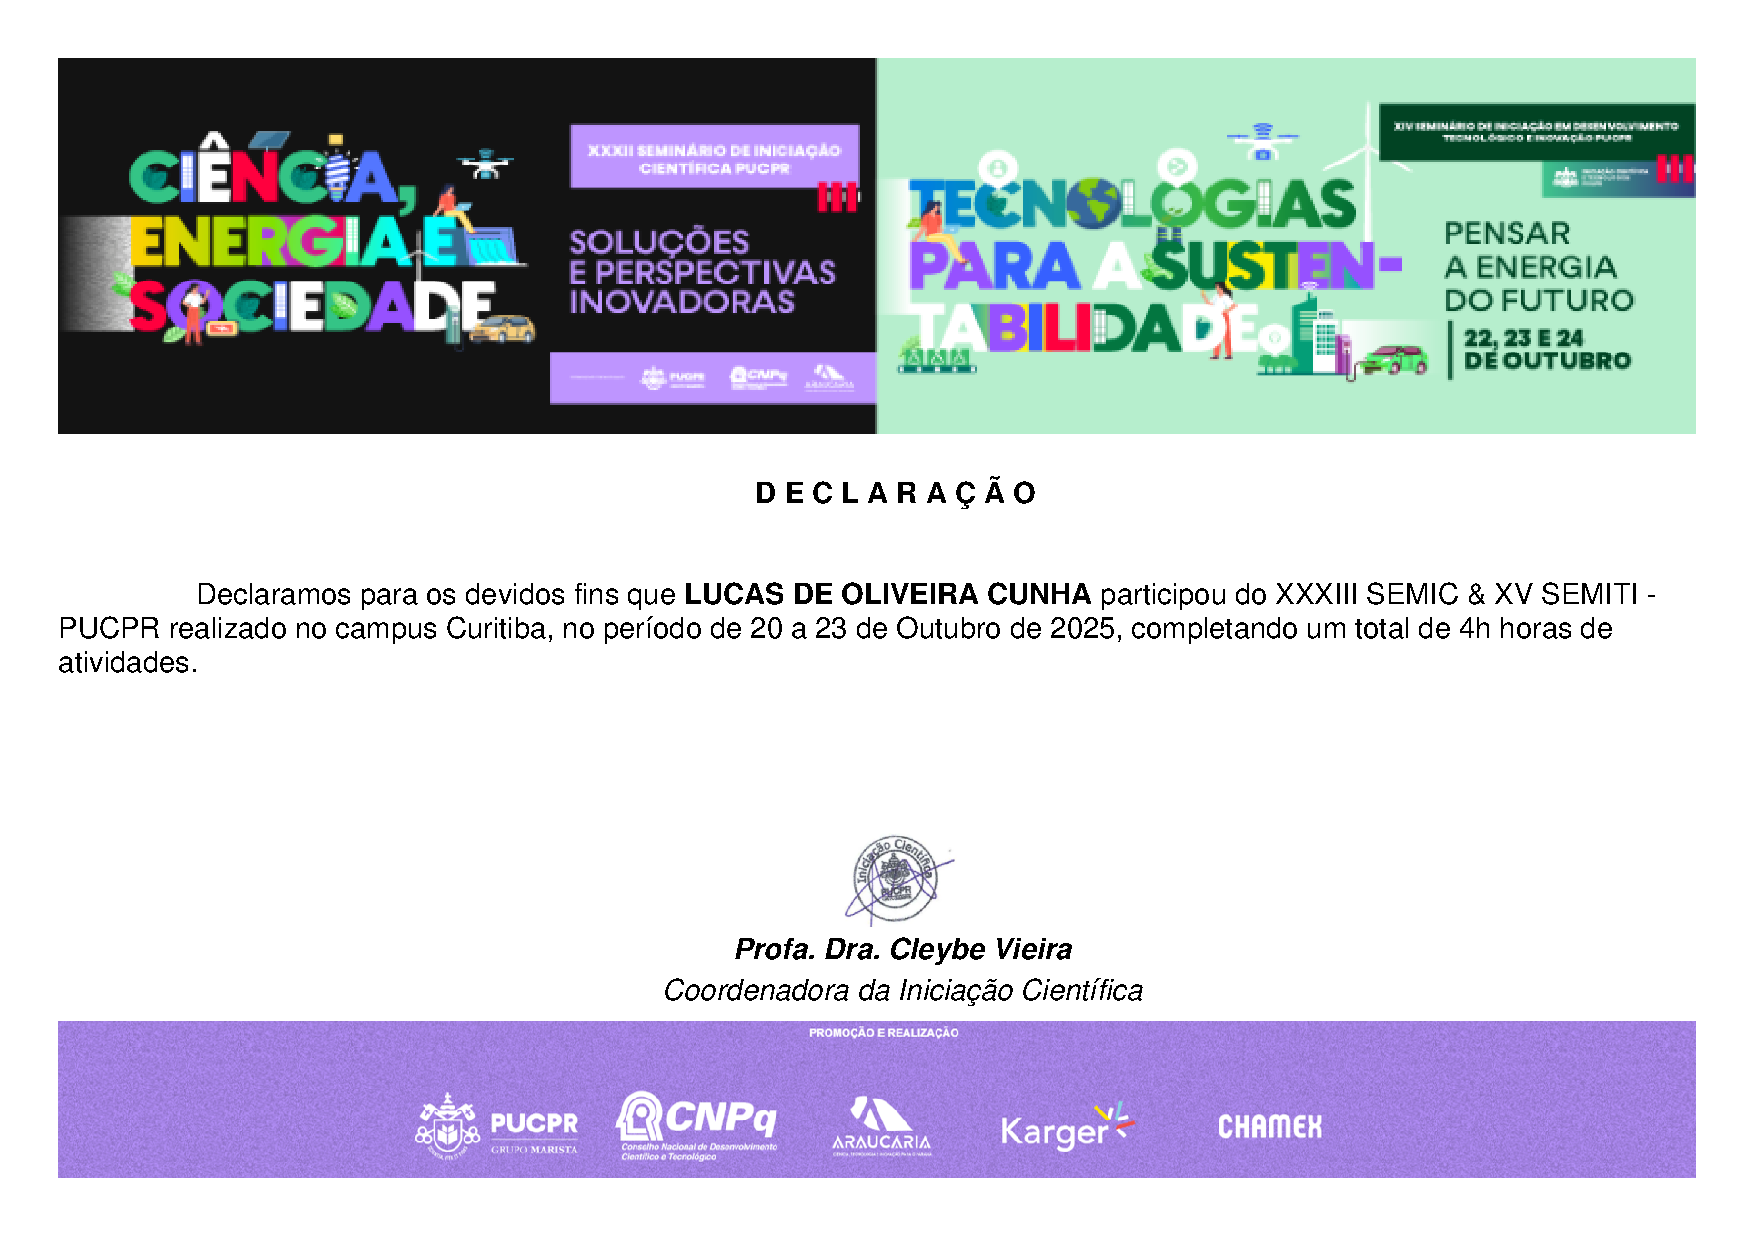
\includegraphics[width=0.5\linewidth]{images/certificado_xxxiii-semic-xv-semiti-pucpr_LUCAS (1).pdf}
\end{figure}

\begin{figure}[H]
    \centering
    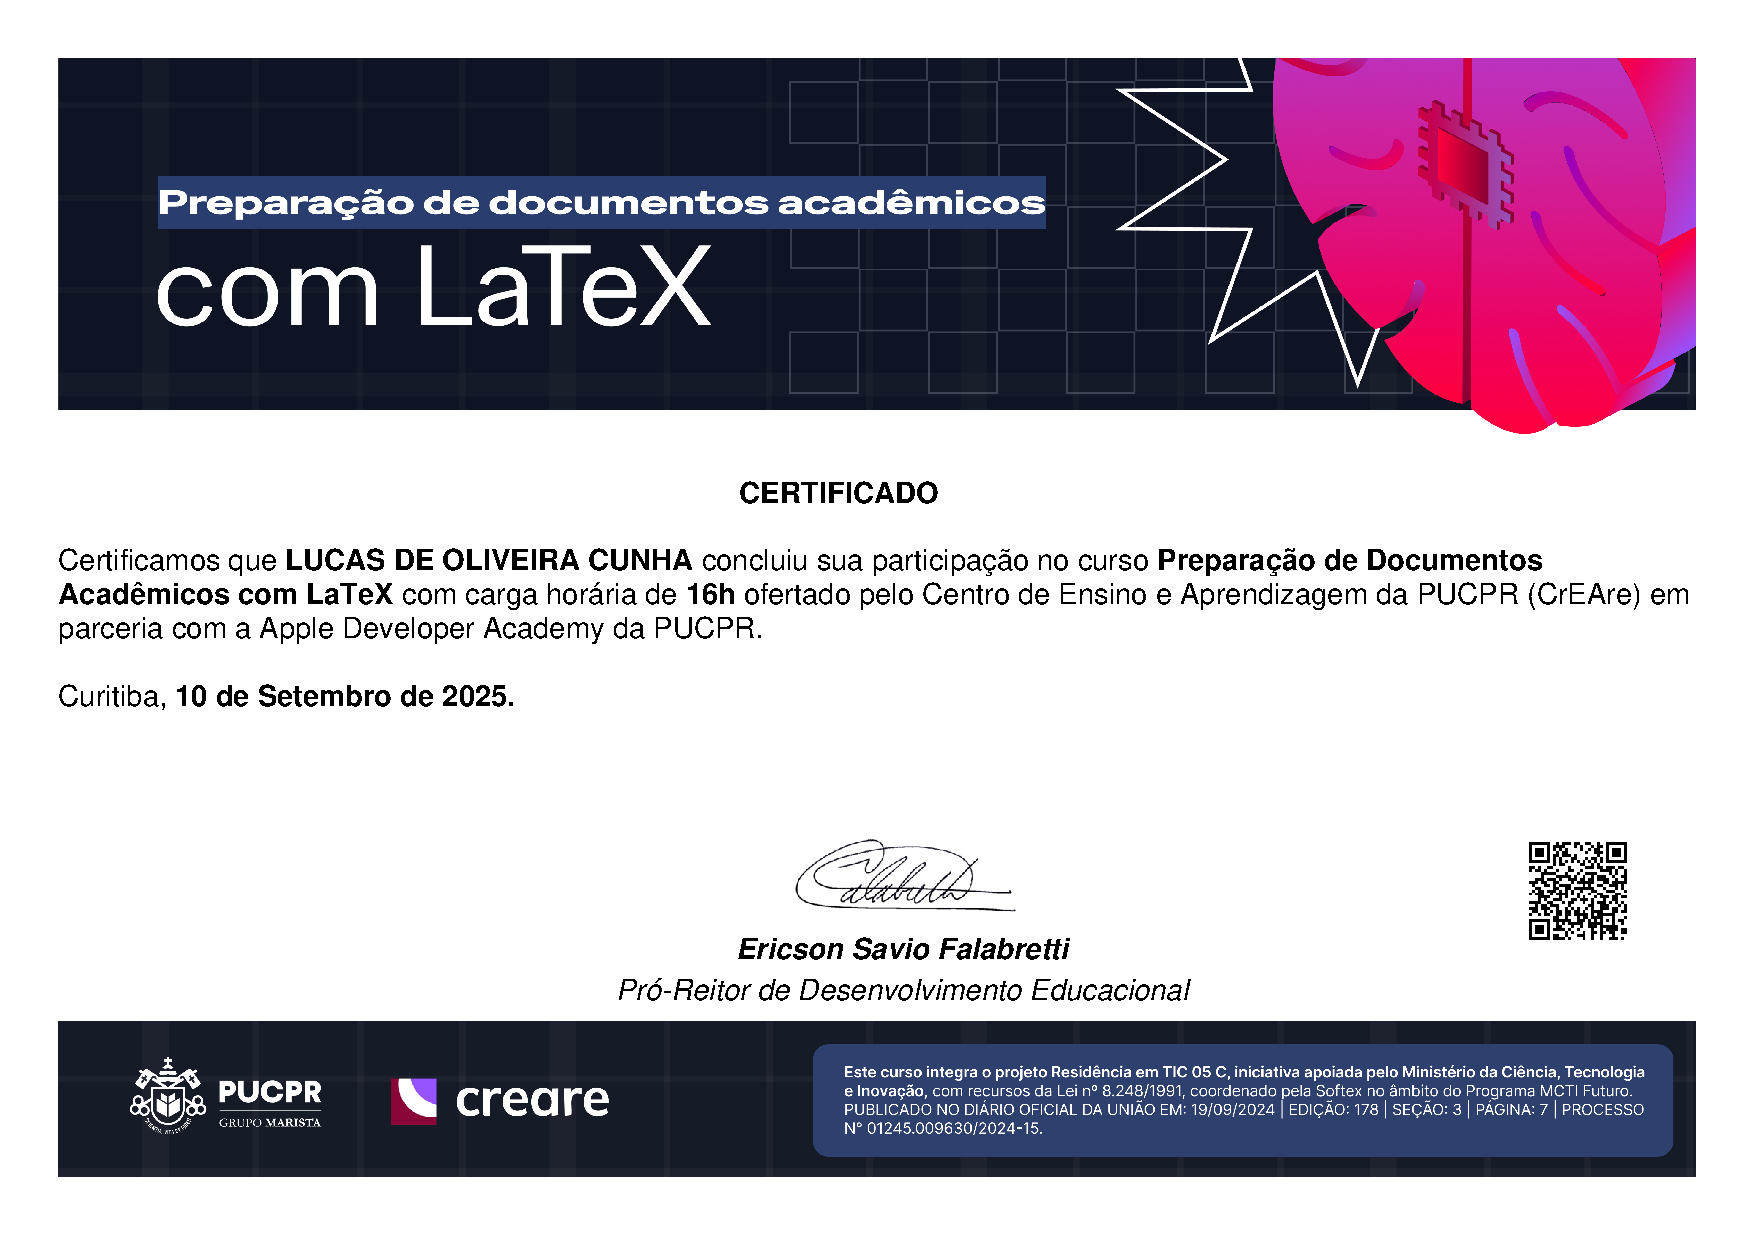
\includegraphics[width=0.5\linewidth]{images/certificado_Preparacao-de-Documentos-Academicos-com-LaTeX-2edicao_LUCAS.pdf}
\end{figure}

\end{document}